\documentclass[ ../main.tex]{subfiles}
\providecommand{\mainx}{..}
\begin{document}
\section{Abstract data type of random approximate sets}
\label{sec:adt}
A \emph{type} is a set and the elements of the set are called the \emph{values} of the type. An \emph{abstract data type} is a type and a set of operations on values of the type.
For example, the \emph{integer} abstract data type is defined by the set of integers and standard operations like addition and subtraction.

A \emph{data structure} is a particular way of organizing data and may implement one or more abstract data types.
Two different data structures that implement the abstract data type should be \emph{exchangable} in a computer program without changing the outward behavior of the program.

See \cref{sec:impl} to see how a C++ interface for the random approximate set data type may be defined.
A popular implementation of an algorithm and data structure that generates approximate sets consistent with the model is known as the \emph{Bloom filter}.

\section{Deterministic algorithm}
By \cref{thm:fpr,thm:fnr}, each independent observation of $\ASet{S}$ generates an uncertain number of false positives and false negatives.
In practice, this may or may not be the case.

Suppose we have a deterministic algorithm that generates approximate sets with a specified expected false positive rate $\fprate$ and false negative rate $\fnrate$.
The algorithm, being deterministic, necessarily generates a certain set $\Set{X}$ given an objective set $\Set{S}$. That is to say, the algorithm is a \emph{total function},
	$\operatorname{f} \colon \PowerSet(\Set{U}) \mapsto \PowerSet(\Set{U})$,
with an \emph{image}
\begin{equation}
\Image(\operatorname{f}) = 
    \SetBuilder{\operatorname{f}(\Set{A})}{\Set{A} \in \PowerSet(\Set{U})}
        \subseteq \PowerSet(\Set{U})\,.
\end{equation}
Since the function $\operatorname{f}$ may map more than one input to the same output, and some sets in the codomain may not be mapped to by any set in the domain, $\operatorname{f}$ is (possibly) a non-surjective, non-injective function.

\subsection{Algebraic properties}
The only thing we can say with certainty \emph{a priori}\footnote{A priori knowledge is independent of experience.} about the image of $\operatorname{f}$ is that its members are subsets of $\Set{U}$ and it contains the empty set $\EmptySet$ and universal set $\Set{U}$.
\begin{definition}
A $\sigma$-algebra is closed under...
\end{definition}
The image of $\operatorname{f}$ is not necessarily a $\sigma$-algebra.
However, the subsets of $\Set{U}$ that may be constructed by countable complements, unions, and intersections for elements of the image is by definition a $\sigma$-algebra and is denoted by $\sigma(\operatorname{f})$.

Since $\sigma(\operatorname{f})$ is a set of sets closed under unions, intersections, and complements, it is a Boolean algebra defined by the six-tuple 
$\left(
    \sigma(\operatorname{f}), \cup, \cap, \SetComplement, \EmptySet,\Set{U}
\right)$,
e.g., set-theoretic operations over the above Boolean algebra are of the form
\begin{equation}
    \sigma(\operatorname{f}) \times \sigma(\operatorname{f}) 
        \mapsto \sigma(\operatorname{f})\,.
\end{equation}
Note that neither \emph{positive} nor \emph{negative} approximate sets are closed under complementation and thus are not Boolean algebras, but rather semi-rings under unions and intersections.

Suppose we have two distinct Boolean algebras,
$\left(
    \sigma(\operatorname{f}), \cup, \cap, \SetComplement, \EmptySet,\Set{U}
\right)$ and 
$\left(
    \sigma(\operatorname{g}), \cup, \cap, \SetComplement, \EmptySet,\Set{U}
\right)$,
where $\operatorname{f}$ and $\operatorname{g}$ are distinct deterministic algorithms that generate approximate sets for $\PowerSet(\Set{U})$.
Set-theoretic operations over both Boolean algebras is the Boolean algebra
$\left(
    \Sigma_{f \cup g}, \cup, \cap, \SetComplement, \EmptySet,\Set{U}
\right)$,
where $\Sigma_{f \cup g} = 
    \sigma\!\left(\sigma(\operatorname{f}) \cup \sigma(\operatorname{g})
\right)$.
Note that $\sigma(\operatorname{f}), \sigma(\operatorname{g}) 
    \subseteq \Sigma_{f \cup g}$,
so if we take the limit
    $\lim_{n \to \infty} \Sigma_{f_1 \cup \cdots \cup f_n}$,
where $f_1,\ldots,f_n$ are distinct mappings, $\Sigma_{f_1 \cup \cdots \cup f_n}$ converges to $\PowerSet(\Set{U})$.

In practice, it is often trivial to implement a large family of random approximate set generators with distinct Boolean algebras given a single implementation, e.g., ``randomly'' seeding a Bloom filter's hash function. As the size of this family goes to infinity, ``randomly'' selecting one of them each time we generate an approximate set generates a random sample consistent with the probability distribution given by \cref{dummyref}.   

%In some cases, it may be important for each objective set to 
%%%have a unique approximate set. A quantity of $n$ 
%%%%deterministic algorithms will label at least 
%$n$ objective sets differently. Unfortunately, there is no 
%%%guarantee that we can 
%satisfy such a requirement.
%\begin{proof}
%We say that a mapping
%    $\operatorname{p} \colon \sigma(\operatorname{f}) 
%%%\mapsto 
%        \sigma(\operatorname{g})$
%is a homomorphism if for all $\Set{A},\Set{B} \in 
%%%\sigma(\operatorname{f})$,
%\begin{align}
%    \operatorname{p}(\EmptySet) &= \EmptySet\,,\\
%    \operatorname{p}(\Set{U}) &= \Set{U}\,,\\
%    \operatorname{p}(\Set{A} \cup \Set{B}) &= 
%        \operatorname{p}(\Set{A}) \cup 
%%%\operatorname{p}(\Set{B})\,,\\
%    \operatorname{p}(\Set{A} \cap \Set{B}) &= 
%        \operatorname{p}(\Set{A}) \cap 
%%%\operatorname{p}(\Set{B})\,.
%\end{align}
%Consider two distinct $\sigma$-algebras 
%%%$\sigma(\operatorname{f})$ and 
%$\sigma(\operatorname{g})$ for $\PowerSet(\{0,1\})$. Suppose 
%%%$\operatorname{f}(\{0\}) = \EmptySet$, 
%%%%$\operatorname{f}(\{0,1\}) = \{0,1\}$, 
%%%%%$\operatorname{g}(\{0\}) = \{0\}$, and 
%%%%%%$\operatorname{g}(\{0,1\}) = \{0,1\}$. Then, 
%%%%%%%$\operatorname{f}(\{0\} \cup \{1\}) = $.
%\end{proof}

%The probability that a particular set is in the 
%%%$\sigma$-algebra is given by the
%probabilistic model. We are not necessarily interested in 
%%%performing this 
%computation. In fact, we are also not interested in 
%assigning %probabilities to 
%the sets in the $\sigma$-algebra; it is not even clear what 
%%%this would mean. 
%Rather, we wish to explore the \emph{algebraic properties} 
%of the approximate set model over a deterministic algorithm.
% PRODUCT sigma-algebra, cartesian products generate product sigma-algebras. This is needed for approximate
% relations paper!
%
%Let {\displaystyle (X_{1},\Sigma _{1})} (X_{1},\Sigma _{1}) and {\displaystyle (X_{2},\Sigma _{2})} (X_{2},\Sigma _{2}) be two measurable spaces. The $\sigma$-algebra for the corresponding product space {\displaystyle X_{1}\times X_{2}} X_{1}\times X_{2} is called the product $\sigma$-algebra and is defined by
%{\displaystyle \Sigma _{1}\times \Sigma _{2}=\sigma (\{B_{1}\times B_{2}:B_{1}\in \Sigma _{1},B_{2}\in \Sigma %_{2}\}).} \Sigma _{1}\times \Sigma _{2}=\sigma (\{B_{1}\times B_{2}:B_{1}\in \Sigma _{1},B_{2}\in \Sigma %_{2}\}).
%$\operatorname{F} \colon [0,1] \times [0,1] \times \PowerSet{U} \mapsto \PowerSet{U}$
%For a given false positive and false negative rate, we may construct a function
%$\operatorname{f} \colon \PowerSet{U} \mapsto \PowerSet{U}$
%$\operatorname{f}(\Set{X} ; \fprate, \fnrate) = \operatorname{F}(\fprate,\fnrate,\Set{X})$

\subsection{Compatibility with the probabilistic model}
How do we reconcile the fact that the algorithm is a \emph{function} with the 
\emph{probabilistic model}? In this context, the notion of \emph{probability} 
quantifies our \emph{ignorance}:
\begin{enumerate}
\item Given an objective set $\Set{S}$, we do not have complete \emph{a priori} 
knowledge about the set $\Set{X}$ it maps to (the approximate set model only 
provides \emph{a priori} knowledge about the probability distribution 
$\ASet{S}$). We acquire \emph{a posterior} knowledge\footnote{A posteriori 
knowledge is dependent on experience.} by applying the algorithm and 
\emph{observing} $\Set{X}$ as its output.
\item Given a set $\Set{X}$ that approximates some unknown objective set 
$\Set{S}$, we do not have complete \emph{a priori} knowledge about $\Set{S}$. 
According to the probabilistic model, the only \emph{a priori} knowledge we have 
is given by the specified \emph{expected} false positive and false negative 
rates. We may acquire a posteriori knowledge by applying the algorithm to each 
set in $\PowerSet(\Set{U})$ and remembering the sets that map to 
$\Set{X}$.\footnote{If the approximate set is the result of the union, 
intersection, and complement of two or more approximate sets, then we must 
consider the closure.}
However, since $\operatorname{f}$ is (possibly) non-injective, one or more sets 
may map to $\Set{X}$ and thus this process may not completely eliminate 
uncertainty. Additionally, the domain $\PowerSet(\Set{U})$ has a cardinality
$2^{\Card{\Set{U}}}$ and thus exhaustive maps are impractical to compute even 
for relatively small domains.\footnote{In the case of \emph{countably infinite} 
domains, it is not even theoretically possible.} However, we may still reduce 
our uncertainty by mapping some subset of interest.
\end{enumerate}

Suppose $\Set{U}$ is finite. There are $2^{\Card{\Set{U}}}$ subsets of
$\Set{U}$, and each set in $\SetDiff[\PowerSet(\Set{U})][\{\EmptySet,\Set{U}\}]$ 
may map (assuming both false positives and false negatives are possible) to 
\emph{any} of subset. There are a total of
\begin{equation}
    2^{2(\Card{\Set{U}} - 1)}
\end{equation}
possible functions that map perform this 
mapping.\footnote{There are a countably infinite number of 
algorithms that may carry out the computations that 
implement any particular function.} Each of these functions 
is compatible with the probabilistic model. For instance, a 
Bloom filter (positive approximate set) may have a family of 
hash function that, for a particular binary coding of the 
elements of a given universal set, maps \emph{every} element 
in the universal set to the same hash. Thus, for instance, no 
matter the objective set $\Set{X} \subseteq \Set{U}$, it will 
map to $\Set{U}$. The Bloom filter had a theoretically sound 
implementation, but only after empirical evidence was it 
discovered that it was not suitable. This is an extremely 
unlikely outcome in the case of large universal sets, but as 
the cardinality of the universal set decreases, the 
probability of such an outcome increases. Indeed, at 
$\Card{U} = 2$, the probability of this outcome is $?$.

Thus, \emph{a priori} knowledge, e.g., a theoretically sound 
algorithm, is not in practice sufficient (although for large 
universal sets, the probability is negligible). The 
suitability of an algorithm can only be determined by 
acquring \emph{a posterior} knowledge.

We could explore the space of functions in the family and 
only choose those which, on some sample of objective sets of 
interest, generates the desired expectations for the false 
positive and false negative rates with the desired variances. 
Most of them will if constructed in the right sort of way.


A family of functions that are compatible with the 
probabilistic model is given by observing a particular 
realization $\Set{X} = \ASet{S}$ and outputting 
$\Set{X}$ on subsequent inputs of $\Set{S}$, i.e., caching 
the output of a \emph{non-deterministic} process that 
conforms to the probabilistic model. This is essentially how 
well-known implementations like the Bloom filter work, where 
the pseudo-randomness comes from mechanical devices like hash 
functions that approximate random oracles.

The false positive rate of the approximate set corresponding 
to objective set $\Set{X}$ is given by
\begin{equation}
    \fprateob(\Set{X}) = \frac{1}{\n} \sum_{x \in \SetComplement[\Set{X}]} \SetIndicator{\operatorname{f}(\Set{X})}(x)\,,
\end{equation}
where $\n = \Card{\SetComplement[\Set{X}]}$.

Let $\Set{U}_p$ denote the set of objective sets with cardinality $\p$. The 
\emph{mean} false positive rate,
\begin{equation}
    \overline{\fprate} = \frac{1}{\Card{\Set{U}_p}}
        \sum_{\Set{X} \in \Set{U}_p} \fprateob(\Set{X})\,,
\end{equation}
is an unbiased estimator of $\fprate$ and the population variance
\begin{equation}
    s^2_\fprate = \frac{1}{\Card{\Set{U}_p}}
        \sum_{\Set{X} \in \Set{U}_p} \fprateob(\Set{X})\,,
\end{equation}
is an unbiased estimator of $\Var{\FPR_\n} = \fprate(1-\fprate)/\n$.
\begin{proof}
We imagine that the function $\operatorname{f}$ caches the output of a 
\emph{non-deterministic} process that conforms to the probabilistic model. Thus, 
each time the function maps an objective set $\Set{X}$ of cardinality $\p$ to 
its approximation, the algorithm \emph{observes} a realization of 
$\FPR_\n = \fprateob$. Thus,
\begin{align}
    \overline{\fprate}
        &= \frac{1}{\Card{\Set{U}_p}} 
            \sum_{\Set{X_i} \in \Set{U}_p} \fprateob(\Set{X}_i)\\
        &= \frac{1}{\Card{\Set{U}_p}} 
            \sum_{\Set{X_i} \in \Set{U}_p} \Expect{\FPR_\n^{(i)}} = \fprate\,.
\end{align}
\end{proof}

\section{Space complexity}
\label{sec:space_comp}
If the finite cardinality of a universe is $u$ and the set is \emph{dense} (and 
the approximation is also dense, i.e., the false negative rate is relatively 
small), then
\begin{equation}
    \mathcal{O}(u) \; \si{bits}
\end{equation}
are needed to code the set, which is independent of $m$, the false positive 
rate, and the false negative rate.

The lower-bound on the \emph{expected} space complexity of a data structure 
implementing the \emph{approximate set} abstract data type where the elements 
are over a \emph{countably infinite} universe is given by the following 
postulate.
\begin{postulate}
\label{pst:approx_l_b}
The \emph{information-theoretic lower-bound}\index{information-theoretic 
lower-bound} of a data structure that implements the countably infinite 
\emph{approximate set} abstract data type has an \emph{expected} bit length 
given by
\begin{equation}
    -(1 - \fnrate) \log_2 \fprate \; \si{bits \per element}\,,
\end{equation}
where $\fprate > 0$ is the false positive rate\index{false positive rate} and 
$\fnrate$ is the false negative rate\index{false negative rate}.
\end{postulate}

The \emph{relative space efficiency}\index{relative space efficiency} of a data 
structure\index{data structure} $X$ to a data structure $Y$ is some value 
greater than $0$ and is given by the ratio of the bit length of $Y$ to the bit 
length of $X$,
\begin{equation}
    \RE(X,Y) = \frac{\BL(Y)}{\BL{X}}\,,
\end{equation}
where $\BL$ is the bit length function. If $\RE(X,Y) < 1$, $X$ is less efficient 
than $Y$, if $\RE(X,Y) > 1$, $X$ is more efficient than $Y$, and if 
$\RE(X,Y) = 1$, $X$ and $Y$ are equally efficient. The absolute space efficiency 
is given by the following definition.
\begin{definition}
The absolute space efficiency of a data structure $X$, denoted by 
\AbsoluteEfficiency{$X$}, is some value between $0$ and $1$ and is given by the 
ratio of the bit length of the theoretical lower-bound to the bit length of $X$,
\begin{equation}
    \AbsoluteEfficiency(X) = \frac{\ell}{\BL(X)}\,,
\end{equation}
where $\BL(X)$ denotes the bit length of $X$ and $\ell$ denotes the bit length 
of the information-theoretic lower-bound. The closer $\AbsoluteEfficiency(X)$ is 
to $1$, the more space-efficient the data structure. A data structure that 
obtains an efficiency of $1$ is \emph{optimal}.\footnote{Sometimes, a data 
structure may only obtain the information-theoretic lower-bound with respect to 
the limit of some parameter, in which case the data structure 
\emph{asymptotically} obtains the lower-bound with respect to said parameter.}
\end{definition}

The \emph{absolute} space efficiency of a data structure $X$ implementing an 
approximate set $\ASet{S}$ with a false positive rate $\fprate$ and false 
negative rate $\fnrate$ is given by
\begin{equation}
    \AbsoluteEfficiency(X) = \frac{-m(1 - \fnrate)\log_2 \fprate}{\BL(X)}\,,
\end{equation}
where $m = \Card{\Set{S}}$. The most useful sort of asymptotic optimality is 
with respect to the parameter $m$.

A well-known implementation of countably infinite \emph{positive approximate 
set} is the Bloom filter\cite{bf} which has an expected space complexity given 
by
\begin{equation}
    -\frac{1}{\ln 2} \log_2 \fprate \; \si{bits \per element}\,,
\end{equation}
thus the absolute efficiency of the Bloom filter is $\ln 2 \approx 0.69$. 
A practical implementation of the \emph{positive approximate set} abstract data 
type is given by the \emph{Perfect Hash Filter}\cite{phf}, which compares 
favorably to the Bloom filter in may circumstances.

The \emph{Singular Hash Set}\cite{shs} is a \emph{theoretical} data structure 
that optimally implements the abstract data types of the \emph{approximate set} 
and the \emph{oblivious set}\cite{obset} abstract data types.

\subsection{Space efficiency of \emph{unions} and \emph{differences}}
As a way to implement \emph{insertions} and \emph{deletions}, we consider the 
space efficiency of the set-theoretic operations of unions and differences of 
approximate sets.

Let $\Set{S}[1] = \{x_{j_1}, \ldots, x_{j_m}\}$ and suppose we wish to insert 
the elements $x_{k_1},\ldots,x_{k_p}$ into $\Set{S}[1]$. If $X_1$ is a mutable 
object, then an \emph{insertion} operator may be applied on $X_1$ for each 
$x_{k_i}$, $i=1,\ldots, p$.

Alternatively, if $X_1$ is immutable, then we may construct another object, 
$X_2$, that implements the set $\Set{S}[2] = \{x_{k_1},\ldots, x_{k_p}\}$, and 
then apply the union function,
\begin{equation}
    \SetUnion[X_1][X_2]\,.
\end{equation}
If we replace $X_1$ and $X_2$ by objects that implement \emph{positive 
approximate sets} of $\Set{S}[1]$ and $\Set{S}[2]$ respectively, then by 
\cref{dummyref}, the false positive rate of the resulting approximate set is 
$\fprateob_1 + \fprateob_2 - \fprateob_1 \fprateob_2$.

The space efficiency of this positive approximate set is given by the following 
theorem.
\begin{theorem}
\label{thm:union_space_complexity}
Given two countably infinite positive approximate sets $\PASet{S}[1]$ and 
$\PASet{S}[2]$ respectively with false positive rates $\fprateob_1$ and 
$\fprateob_2$, the approximate set $\SetUnion[\PASet{S}[1]][\PASet{S}[2]]$, 
which has an induced false positive rate 
    $\fprateob_1 + \fprateob_2 - \fprateob_1 \fprateob_2$,
has an expected upper-bound on its absolute efficiency given by
\begin{equation}
\label{eq:union_space_complexity}
    \AbsoluteEfficiency(\fprateob_1, \fprateob_2 \Given \alpha_1, \alpha_2) =
    \frac{
        \log_2\!\left(
        \fprateob_1 + \fprateob_2 - \fprateob_1 \fprateob_2
        \right)}
        {
            \alpha_1 \log_2 \fprateob_1 + \alpha_2 \log_2 \fprateob_2
        }\,,
\end{equation}
where
\begin{equation}
\label{eq:union_space_complexity_bounds}
\begin{split}
    0 &< \alpha_1 = \frac{\Card{\Set{S}[1]}}
        {\Card{\SetUnion[\Set{S}[1]][\Set{S}[2]]}} \leq 1\,,\\
    0 &< \alpha_2 = \frac{\Card{\Set{S}[2]}}
        {\Card{\SetUnion[\Set{S}[1]][\Set{S}[2]]}} \leq 1\,,\\
    1 &\leq \alpha_1 + \alpha_2\,.
\end{split}
\end{equation}
As $\fprateob_j \to 1$ or $\fprateob_j \to 0$ for $j=1,2$, or 
    $(\fprateob_1, \fprateob_2) \to (1,1)$, 
the absolute efficiency goes to $0$.
\footnote{As $(\fprateob_1,\fprateob_2) \to (0,0)$, the absolute efficiency 
depends on the path taken. In most cases, it goes to $0$.}
\end{theorem}
\begin{proof}
The proof comes in two parts. First, we prove \cref{eq:union_space_complexity}, 
and then we prove the bounds on $\alpha_1$ and $\alpha_2$ given by 
\cref{eq:union_space_complexity_bounds}.

Let $X$ and $Y$ denote optimally space-efficient data structures that 
respectively implement positive approximate sets $\PASet{S}[1]$ and 
$\PASet{S}[2]$ with false positive rates $\fprateob_1$ and $\fprateob_2$. By 
\cref{dummyref}, their union has an induced false positive rate given by
\begin{equation}
    \fprateob_1 + \fprateob_2 + \fprateob_1 \fprateob_2\,.
\end{equation}
The information-theoretic lower-bound of the approximate set of 
$\SetUnion[\Set{S}[1]][\Set{S}[2]]$ with the above false positive rate is given 
by
\begin{equation}
    -\Card{\SetUnion[\Set{S}[1]][\Set{S}[2]]}
        \log_2 \! \left(\fprateob_1 + \fprateob_2 +
        \fprateob_1 \fprateob_2\right) \; \si{bits}\,.
\end{equation}
Since we assume we only have $X$ and $Y$ and it is not possible to enumerate the 
elements in either, we must implement their union by storing and separately 
querying both $X$ and $Y$. Since $X$ and $Y$ are optimal, 
$\BL(X) = -\Card{\Set{S}[1]} \log_2 \fprateob_1$ and 
$\BL(Y) = -\Card{\Set{S}[2]} \log_2 \fprateob_2$. 
Making these substitutions yields an absolute efficiency ???
\begin{equation}
\label{eq:proof_union_ae}
    \AbsoluteEfficiency = \frac{\Card{\SetUnion[\Set{S}[1]][\Set{S}[2]]} \log_2 \! \left(\fprateob_1 + \fprateob_2 + \fprateob_1 \fprateob_2\right)}{\Card{\Set{S}[1]} \log_2 \fprateob_1 + \Card{\Set{S}[2]} \log_2 \fprateob_2}\,.
\end{equation}
Letting
\begin{equation}
    \alpha_1 = \frac{\Card{\Set{S}[1]}}{\Card{\SetUnion[\Set{S}[1]][\Set{S}[2]]}} \; \text{and} \; \alpha_2 = \frac{\Card{\Set{S}[2]}}{\Card{\SetUnion[\Set{S}[1]][\Set{S}[2]]}}\,,
\end{equation}
we may rewrite \cref{eq:proof_union_ae} as
\begin{equation*}
    \frac{
        \log_2\!\left(\fprateob_1 + \fprateob_2 - \fprateob_1 \fprateob_2\right)}
    {
        \alpha_1 \log_2 \fprateob_1 + \alpha_2 \log_2 \fprateob_2
    }\,.\tag{\ref{eq:union_space_complexity} revisited}
\end{equation*}

In the second part of the proof, we prove the bounds on $\alpha_1$ and $\alpha_2$ as given by \cref{eq:union_space_complexity_bounds}.
Both $\alpha_1$ and $\alpha_2$ must be non-negative since each is the ratio of two positive numbers (cardinalities). If $\Card{\Set{S}[1]} \ll \Card{\Set{S}[2]}$, then $\alpha_1 \approx 0$. If $\Set{S}[1] \supset \Set{S}[2]$, then $\alpha_1 = 1$. A similar argument holds for $\alpha_2$. Finally,
\begin{equation}
    \alpha_1 + \alpha_2 = \frac{\Card{\Set{S}[1]} + \Card{\Set{S}[2]}}{\Card{\SetUnion[\Set{S}[1]][\Set{S}[2]]}}
\end{equation}
has a minimum value by assuming that $\Set{S}[1]$ and $\Set{S}[2]$ are disjoint sets (i.e., their intersection is the empty set), in which case
\begin{equation}
    \alpha_1 + \alpha_2 = \frac{\Card{\Set{S}[1]} + \Card{\Set{S}[2]}}{\Card{\Set{S}[1]} + \Card{\Set{S}[2]}} = 1\,.
\end{equation}
\end{proof}
See \cref{dummyref} for a contour plot of the expected lower-bound as a function of $\fprateob_1$ and $\fprateob_2$. As $\fprateob_1 \to 0$ or $\fprateob_2 \to 0$, the efficiency goes to $0$.

The lower-bound on the efficiency of the union of approximate sets is given by the following corollary.
\begin{corollary}
Given two positive, non-enumerable approximate sets with false positive rates $\fprateob_1$ and $\fprateob_2$, their union is an approximate set that has an efficiency that is expected to be greater than the lower bound given by
\begin{equation}
    \min \AbsoluteEfficiency(\fprateob_1, \fprateob_2) = \frac{
        \log_2\!\left(\fprateob_1 + \fprateob_2 - \fprateob_1 \fprateob_2\right)}
    {
        \log_2 \fprateob_1 \fprateob_2
    }\,.
\end{equation}
\end{corollary}


\begin{corollary}
If $\fprate_1 = \fprate_2 = \fprate$, then the absolute efficiency is given by
\begin{equation}
\AbsoluteEfficiency(\fprateob \Given \alpha) = \left(1 + \frac{\log_2(2 - \fprateob)}{\log_2 \fprateob}\right)\left(1 - \frac{\alpha}{2}\right)\,,
\end{equation}
where
\begin{equation}
    0 \leq \alpha = \frac{\Card{\SetIntersection[\Set{S}[1]][\Set{S}[2]]}}{\Card{\SetUnion[\Set{S}[1]][\Set{S}[2]]}} \leq 1\,,
\end{equation}
which is a monotonically decreasing function with respect to $\fprate$ and $\alpha$ with limits given by $\lim_{\fprateob \to 0} \AbsoluteEfficiency(\fprate) = 1$ and $\lim_{\fprate \to 1} \AbsoluteEfficiency(\fprate) = 0$.
\end{corollary}
See \cref{fig:cor_union_same_fprate} for a graphic illustration.

\COMMENT{
\begin{figure}
\centering
\caption{Expected lower-bound on efficiency of the union of two approximate sets, neither of which can be enumerated.}
\begin{tikzpicture}
%\selectcolormodel{gray}
    \begin{axis}
    [
        xmax=.999,
        xmin=.001,
        ymax=.999,
        ymin=.001,
        zmin=0,
        xlabel={$\fprate_1$},
        ylabel={$\fprate_2$},
        zlabel={$\min \AbsoluteEfficiency(\fprate_1,\fprate_2)$},
        axis lines=left,
        ztick=\empty,
        xmode=log,
        ymode=log,
        log ticks with fixed point,
        minor tick style={draw=none}
    ]
    \addplot3[
        contour gnuplot={levels={0.1,0.2,0.3,0.4}},
        domain=.001:.999,
        y domain=.001:.999
    ] {log2(x + y - x * y) / log2(x * y)};
    \end{axis}
\end{tikzpicture}
\label{fig:cor_union_same_fprate}
\end{figure}

\begin{figure}
\label{fig:efficiency_vs_fprate_union_paset}
\centering
\captionsetup{justification=centering}
\caption
{
    The expected false positive rate $\fprate$ vs the expected lower-bound on the absolute space efficiency for the union of two approximate sets where it is not possible to enumerate the elements.
}
\begin{tikzpicture}
\begin{axis}
[
    xmax=1,
    xmin=0,
    ymax=1,
    ymin=0,
    xlabel={$\fprate$},
    ylabel={\AbsoluteEfficiency{$\fprate \Given \alpha$}},
    no markers,
    cycle list={black}
    legend style={nodes=right},
    legend pos={north east}
]
\addlegendentry{\AbsoluteEfficiency{$\fprate \Given \alpha=1$}}
\addplot[solid] table [col sep=comma] {data/data1.csv};
\addlegendentry{\AbsoluteEfficiency{$\fprate \Given \alpha=0.5$}}
\addplot[dashed] table [col sep=comma] {data/data.5.csv};
\addlegendentry{\AbsoluteEfficiency{$\fprate \Given \alpha=0.25$}}
\addplot[dashdotted] table [col sep=comma] {data/data.25.csv};
\addlegendentry{\AbsoluteEfficiency{$\fprate \Given \alpha = 0$}}
\addplot[dotted] table [col sep=comma] {data/efficiency_fprate_union.csv};
\end{axis}
\end{tikzpicture}
\end{figure}
}

\begin{figure}
\centering
\caption{Expected lower-bound on efficiency of the union of two approximate sets with the same false positive rate $\fprate$, neither of which can be enumerated.}
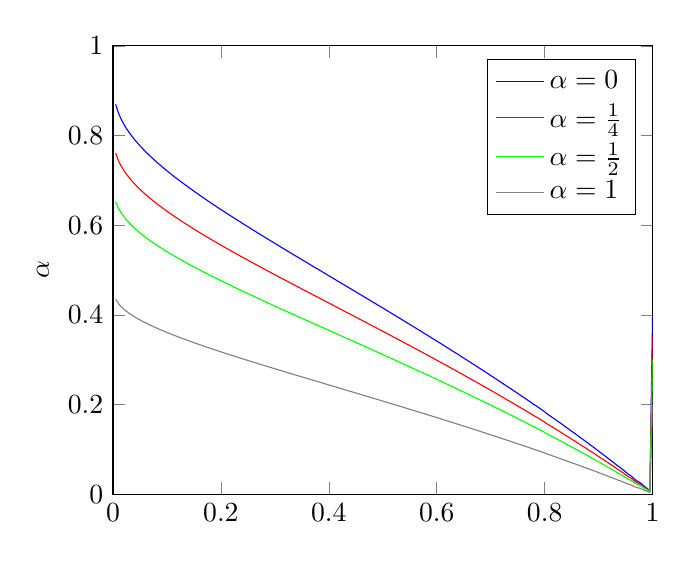
\begin{tikzpicture}
\begin{axis}
[
    xmax=1,
    xmin=0,
    ymax=1,
    ymin=0,
    xlabel={$\fprate$},
    ylabel={\AbsoluteEfficiency{$\fprate \Given \alpha$}},
    %no markers,
    %cycle list={black}
    legend style={nodes=right},
    legend pos={north east}
]
\addlegendentry{\AbsoluteEfficiency{$\fprate \Given \alpha=0$}}
\addplot[blue,domain=0:1,samples=200] {(1 + log2(2-x)/log2(x))};
\addlegendentry{\AbsoluteEfficiency{$\fprate \Given \alpha=\frac{1}{4}$}}
\addplot[red,domain=0:1,samples=200] {(1 + log2(2-x)/log2(x))*(.875)};
\addlegendentry{\AbsoluteEfficiency{$\fprate \Given \alpha=\frac{1}{2}$}}
\addplot[green,domain=0:1,samples=200] {(1 + log2(2-x)/log2(x))*(.75)};
\addlegendentry{\AbsoluteEfficiency{$\fprate \Given \alpha=1$}}
\addplot[gray,domain=0:1,samples=200] {(1 + log2(2-x)/log2(x))/2};
\end{axis}
\end{tikzpicture}
\label{fig:cor_union_same_fprate}
\end{figure}
















\end{document}










